\documentclass[11pt,a4paper]{ctexart}

\usepackage[margin=2.2cm]{geometry}
\usepackage{amsmath,amssymb,bm}
\usepackage{booktabs}
\usepackage{graphicx}
\usepackage{hyperref}
\usepackage{xcolor}
\usepackage{caption}
\usepackage{subcaption}
\usepackage{enumitem}
\usepackage{float}
\usepackage{siunitx}
\usepackage{xurl}

\hypersetup{
  colorlinks=true,
  linkcolor=blue!55!black,
  citecolor=blue!55!black,
  urlcolor=blue!55!black
}

\setlist[itemize]{leftmargin=1.8em}
\setlist[enumerate]{leftmargin=1.8em}
\captionsetup{font=small}
\emergencystretch=3em
\Urlmuskip=0mu plus 2mu

\title{\bfseries 任务五子任务二 Example 4 的运行理解与结果说明\\
\large 空间引力波数据、傅立叶分析、MBHB 信号与贝叶斯推断}
\author{Lei Chang \quad \texttt{task5-lisa-taiji}}
\date{\today}

\begin{document}
\maketitle

\begin{abstract}
中国科学院大学 2026 年科创计划任务五子任务二要求运行并理解
Triangle-BBH 仓库 Examples 文件夹下编号为 4 的示例。本文结合官方
\path{4_TDC_Verification_MBHB_Search_and_Estimation(CPU).ipynb}、
本仓库 \path{notebooks/02_taiji_mbhb_parameter_estimation.ipynb}
的实际运行结果，以及 Taiji Data Challenge、NESSAI 和近两年 LISA/Taiji
MBHB 推断相关开放获取文献，梳理空间引力波探测数据形式、傅立叶变换、
大质量双黑洞并合信号建模和贝叶斯统计推断的关键逻辑。本文的重点不是复述
代码，而是说明每一步为什么必要、输出应如何解释、以及当前结果的可信度边界。
\end{abstract}

\section{任务要求与材料来源}

子任务二的核心要求可以概括为四层：
\begin{enumerate}
  \item 复现并理解 Triangle-BBH 官方 Example 4，即在 Taiji/TDC 数据中完成
  MBHB 信号的搜索、参数估计和结果诊断。
  \item 理解空间引力波数据的形式，包括时域数据、频域数据、TDI 通道和噪声
  功率谱密度。
  \item 理解大质量双黑洞并合（massive black hole binary, MBHB）波形如何进入
  Taiji 响应，并解释天区、距离、倾角等外禀参数中的简并。
  \item 理解贝叶斯统计推断，包括似然、先验、后验、证据、嵌套采样和诊断。
\end{enumerate}

本仓库的 notebook 2 保持了 Example 4 的科学流程：从 TDC 数据读取、TDI
通道处理、FFT/PSD 构造、F 统计搜索、Fisher 局部先验、NESSAI 采样到
后验可视化。与官方 CPU 示例不同，本仓库为了在可交付时间内完成全量采样，
采用 GPU 杂频似然（heterodyned likelihood）接入 NESSAI 的路线。该路线不改变
贝叶斯推断对象，而是将昂贵的全频似然评估替换为参考波形附近的快速近似评估。

\section{Example 4 的主流程理解}

官方 Example 4 可以视为一个完整的参数估计闭环：
\[
  \text{TDC 数据} \rightarrow
  \text{TDI/频域预处理} \rightarrow
  \text{MBHB 搜索} \rightarrow
  \text{局部先验} \rightarrow
  \text{NESSAI 后验采样} \rightarrow
  \text{诊断与物理解释}.
\]
每一步的含义如下。

\paragraph{数据读取。}
TDC 文件以 HDF5 形式保存观测时间序列和注入参数。空间引力波数据不是单一
地面干涉仪应变，而是由三个航天器之间的激光链路经时间延迟干涉
（time-delay interferometry, TDI）组合得到。Example 4 关注的是 MBHB 注入
信号在 Taiji 类探测器数据中的恢复。

\paragraph{TDI 通道。}
原始链路噪声通过 TDI 组合构造成近似独立的探测通道。实际分析常从
\(X,Y,Z\) 组合变换到 \(A,E,T\) 或其中较敏感的 \(A,E\) 通道。对 MBHB 这类
强信号，\(A/E\) 通道既保留主要信号信息，又便于写出多通道频域内积和似然。

\paragraph{搜索与估计的分工。}
F 统计搜索的任务是给出接近最大似然的初值，尤其是天区、相位、时间和质量等
参数的候选区域；NESSAI 的任务则是在先验约束下给出完整后验样本和证据估计。
搜索不是最终结论，采样后验才是参数不确定性的主要来源。

\section{空间引力波数据形式与傅立叶变换}

空间引力波探测器的观测数据可以抽象为
\[
  d_k(t) = h_k(t;\bm{\theta}) + n_k(t), \qquad k \in \{A,E\},
\]
其中 \(h_k\) 是给定参数 \(\bm{\theta}\) 下的探测器响应，\(n_k\) 是噪声。
由于噪声谱随频率变化，似然通常写在频域。离散傅立叶变换将时域序列
\(d(t_j)\) 变为频域序列 \(\tilde d(f_i)\)，随后结合单边噪声功率谱
\(S_{n,k}(f)\) 定义内积
\[
  (a|b) =
  4\,\mathrm{Re}\sum_{k\in\{A,E\}}\sum_i
  \frac{\tilde a_k^*(f_i)\tilde b_k(f_i)}{S_{n,k}(f_i)}\Delta f .
\]
在高斯平稳噪声假设下，频域对数似然可写为
\[
  \log \mathcal{L}(\bm{\theta})
  = -\frac{1}{2}\left(d-h(\bm{\theta})\,\middle|\,d-h(\bm{\theta})\right)
  + C .
\]
因此，FFT、PSD 估计、频段选择和窗函数不是单纯的画图步骤，而是决定似然
数值稳定性的基础。对于长时长空间信号，直接在每个采样点上重新生成全频
波形会非常昂贵，这也是杂频似然能够显著加速的根本原因。

\section{MBHB 信号和 Taiji 响应}

MBHB 信号由内禀参数和外禀参数共同决定。内禀参数包括红移质量、质量比和自旋，
决定 inspiral--merger--ringdown 的相位演化和振幅结构；外禀参数包括天区位置、
倾角、偏振角、光度距离、合并时间和合并相位，决定探测器如何“看见”该波形。

在空间探测器中，轨道运动带来的 Doppler 调制和天线图样调制对天区定位至关重要。
这也解释了本仓库结果中常见的天区反射简并：不同的 ecliptic/探测器框架位置可能
产生相近响应，从而形成主解和反射解两支后验。当前 notebook 2 的全量结果主要落在
反射解附近；这不表示分析错误，而是 Taiji/LISA 类空间探测器中常见的几何简并。
严格比较“直接解”和“反射解”的相对权重，需要分别以两支解为 fiducial 重新构造
杂频似然并比较各自后验和证据。

\section{贝叶斯推断与 NESSAI}

贝叶斯推断的目标是从数据 \(d\) 推断参数 \(\bm{\theta}\)。核心公式是
\[
  p(\bm{\theta}|d)
  = \frac{\mathcal{L}(d|\bm{\theta})\pi(\bm{\theta})}{Z},
  \qquad
  Z = \int \mathcal{L}(d|\bm{\theta})\pi(\bm{\theta})\,d\bm{\theta}.
\]
其中 \(\pi(\bm{\theta})\) 是先验，\(Z\) 是贝叶斯证据。后验样本用于给出参数中位数、
置信区间和相关性；证据可用于同一数据集、不同模型之间的比较。

NESSAI 是基于 normalising flows 的嵌套采样器。它学习 live points 在等似然面内
的分布，并从流模型中提出新样本。对引力波问题而言，NESSAI 的价值在于：当单次
似然评估昂贵时，减少似然调用次数可以抵消训练 flow 的开销；同时，NESSAI 能给出
后验样本、证据和 insertion-index 等诊断。需要注意的是，单次 TDC 注入无法完成
群体意义上的 P--P 检验；本仓库只能报告单次运行内部的 insertion-index 诊断。

\section{本仓库的实现路线}

本仓库的 notebook 2 使用如下策略：
\begin{enumerate}
  \item 保持 Example 4 的科学结构和参数定义。
  \item 使用 GPU F 统计搜索给出候选点，并用 Fisher 信息构造局部先验盒。
  \item 在候选点附近构造 GPU 杂频似然，减少每次似然评估需要处理的频点数量。
  \item 将向量化 GPU 似然包装为 NESSAI model，使用 \(n_\mathrm{live}=2000\)
  做 full run。
  \item 对 baseline 窗口和 5-day 非对称窗口分别运行，并比较后验 CI、天区图、
  corner 图、insertion-index 和边界检查。
\end{enumerate}

这一路线与官方 CPU Example 4 的关系是“同一统计问题、不同计算实现”。官方
示例更接近教学基线；本仓库版本强调在保持 NESSAI 全量采样的同时，将运行时间
压缩到可交付范围。

\section{实际运行结果}

表 \ref{tab:nessai-summary} 汇总了 notebook 2 的两次 full NESSAI 运行。两个窗口
的数据段不同，因此两者的 \(\Delta \log Z\) 不能解释为 Bayes factor；这里的
\(\log Z\) 只作为各自运行的收敛性和内部一致性指标。

\begin{table}[H]
  \centering
  \caption{GPU 杂频似然 + NESSAI full run 结果摘要。}
  \label{tab:nessai-summary}
  \begin{tabular}{lcc}
    \toprule
    指标 & baseline Example 4 窗口 & 5-day 非对称窗口 \\
    \midrule
    \(n_\mathrm{live}\) & 2000 & 2000 \\
    \(\log Z\) & 594014.861 & 594995.406 \\
    \(\sigma_{\log Z}\) & 0.124 & 0.125 \\
    后验样本数 & 10890 & 10879 \\
    wall time & 9.44 min & 9.59 min \\
    insertion-index KS \(p\) & 0.480 & 0.357 \\
    最大边界占比 & 0.0065 & 0.0074 \\
    \bottomrule
  \end{tabular}
\end{table}

从诊断上看，两个窗口的 insertion-index \(p\) 值没有显示明显过约束或欠约束；
边界占比低于 1\%，说明 Fisher 局部先验没有把主要后验截断在边界上。参数方面，
chirp mass 的 90\% 置信区间宽度在 5-day 窗口中约为 baseline 的 0.877，说明延长
有效观测窗口可以改善质量参数约束；光度距离和天区参数受距离--倾角简并及天区
反射简并影响，改善不一定单调。

\begin{table}[H]
  \centering
  \caption{部分参数 90\% 置信区间宽度比较。比值小于 1 表示 5-day 窗口更窄。}
  \label{tab:ci-summary}
  \begin{tabular}{lccc}
    \toprule
    参数 & baseline CI90 宽度 & 5-day CI90 宽度 & 比值 \\
    \midrule
    chirp mass & 8172.59 & 7169.53 & 0.877 \\
    mass ratio & 0.00438 & 0.00414 & 0.944 \\
    spin\_1z & 0.02694 & 0.02649 & 0.983 \\
    spin\_2z & 0.12220 & 0.11914 & 0.975 \\
    luminosity distance & 9950.04 & 10241.14 & 1.029 \\
    longitude & 0.75951 & 0.76594 & 1.008 \\
    latitude & 0.68250 & 0.67582 & 0.990 \\
    \bottomrule
  \end{tabular}
\end{table}

\begin{figure}[H]
  \centering
  \begin{subfigure}{0.48\textwidth}
    \centering
    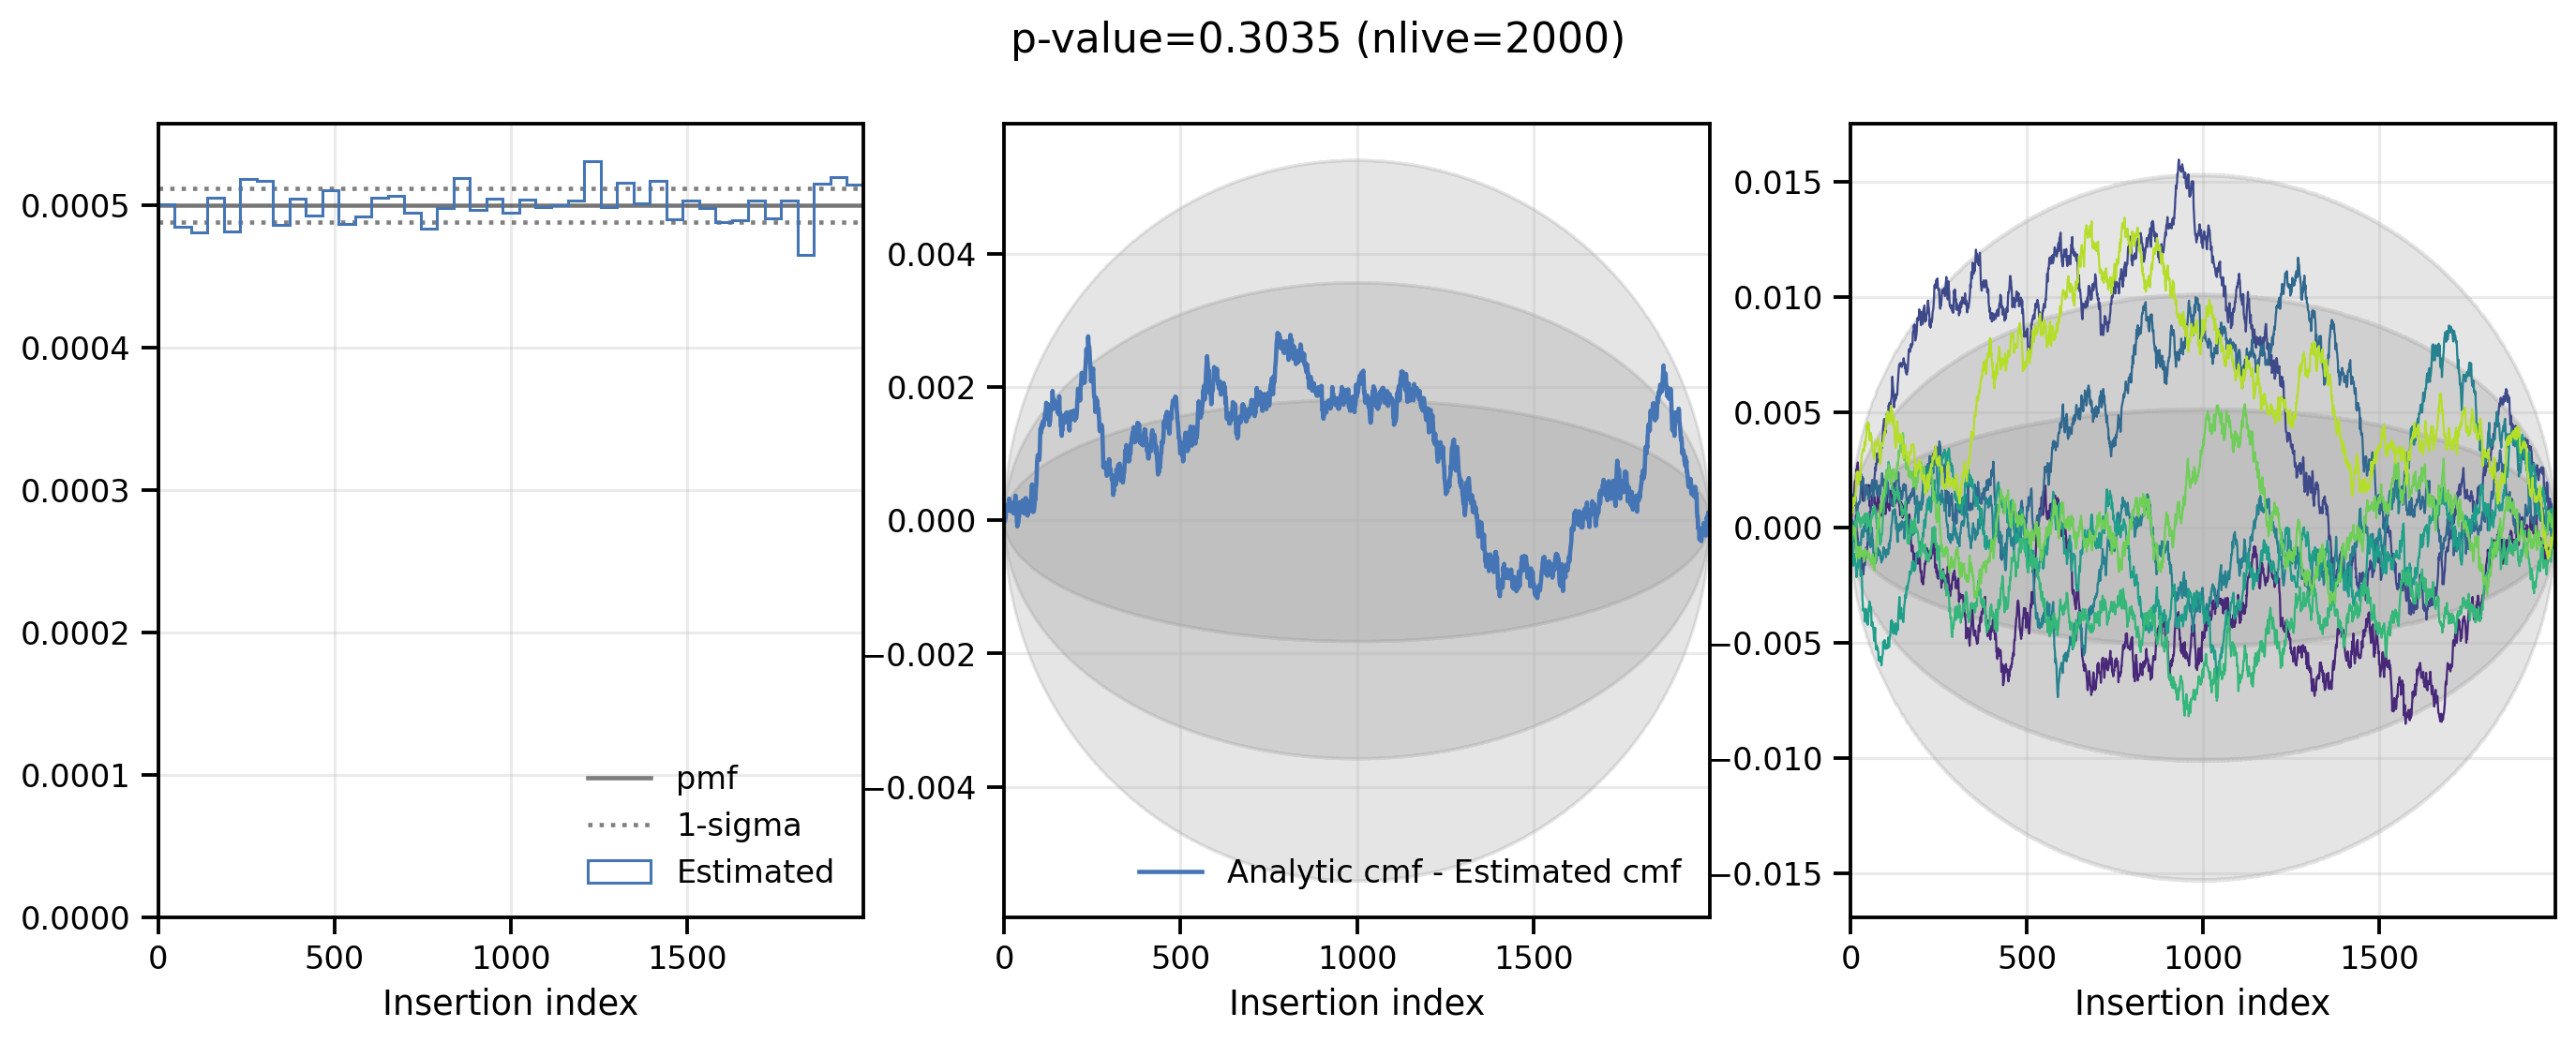
\includegraphics[width=\linewidth]{../figures/task5_subtask2/11_baseline_nessai_insertion_indices.png}
    \caption{baseline insertion-index}
  \end{subfigure}
  \hfill
  \begin{subfigure}{0.48\textwidth}
    \centering
    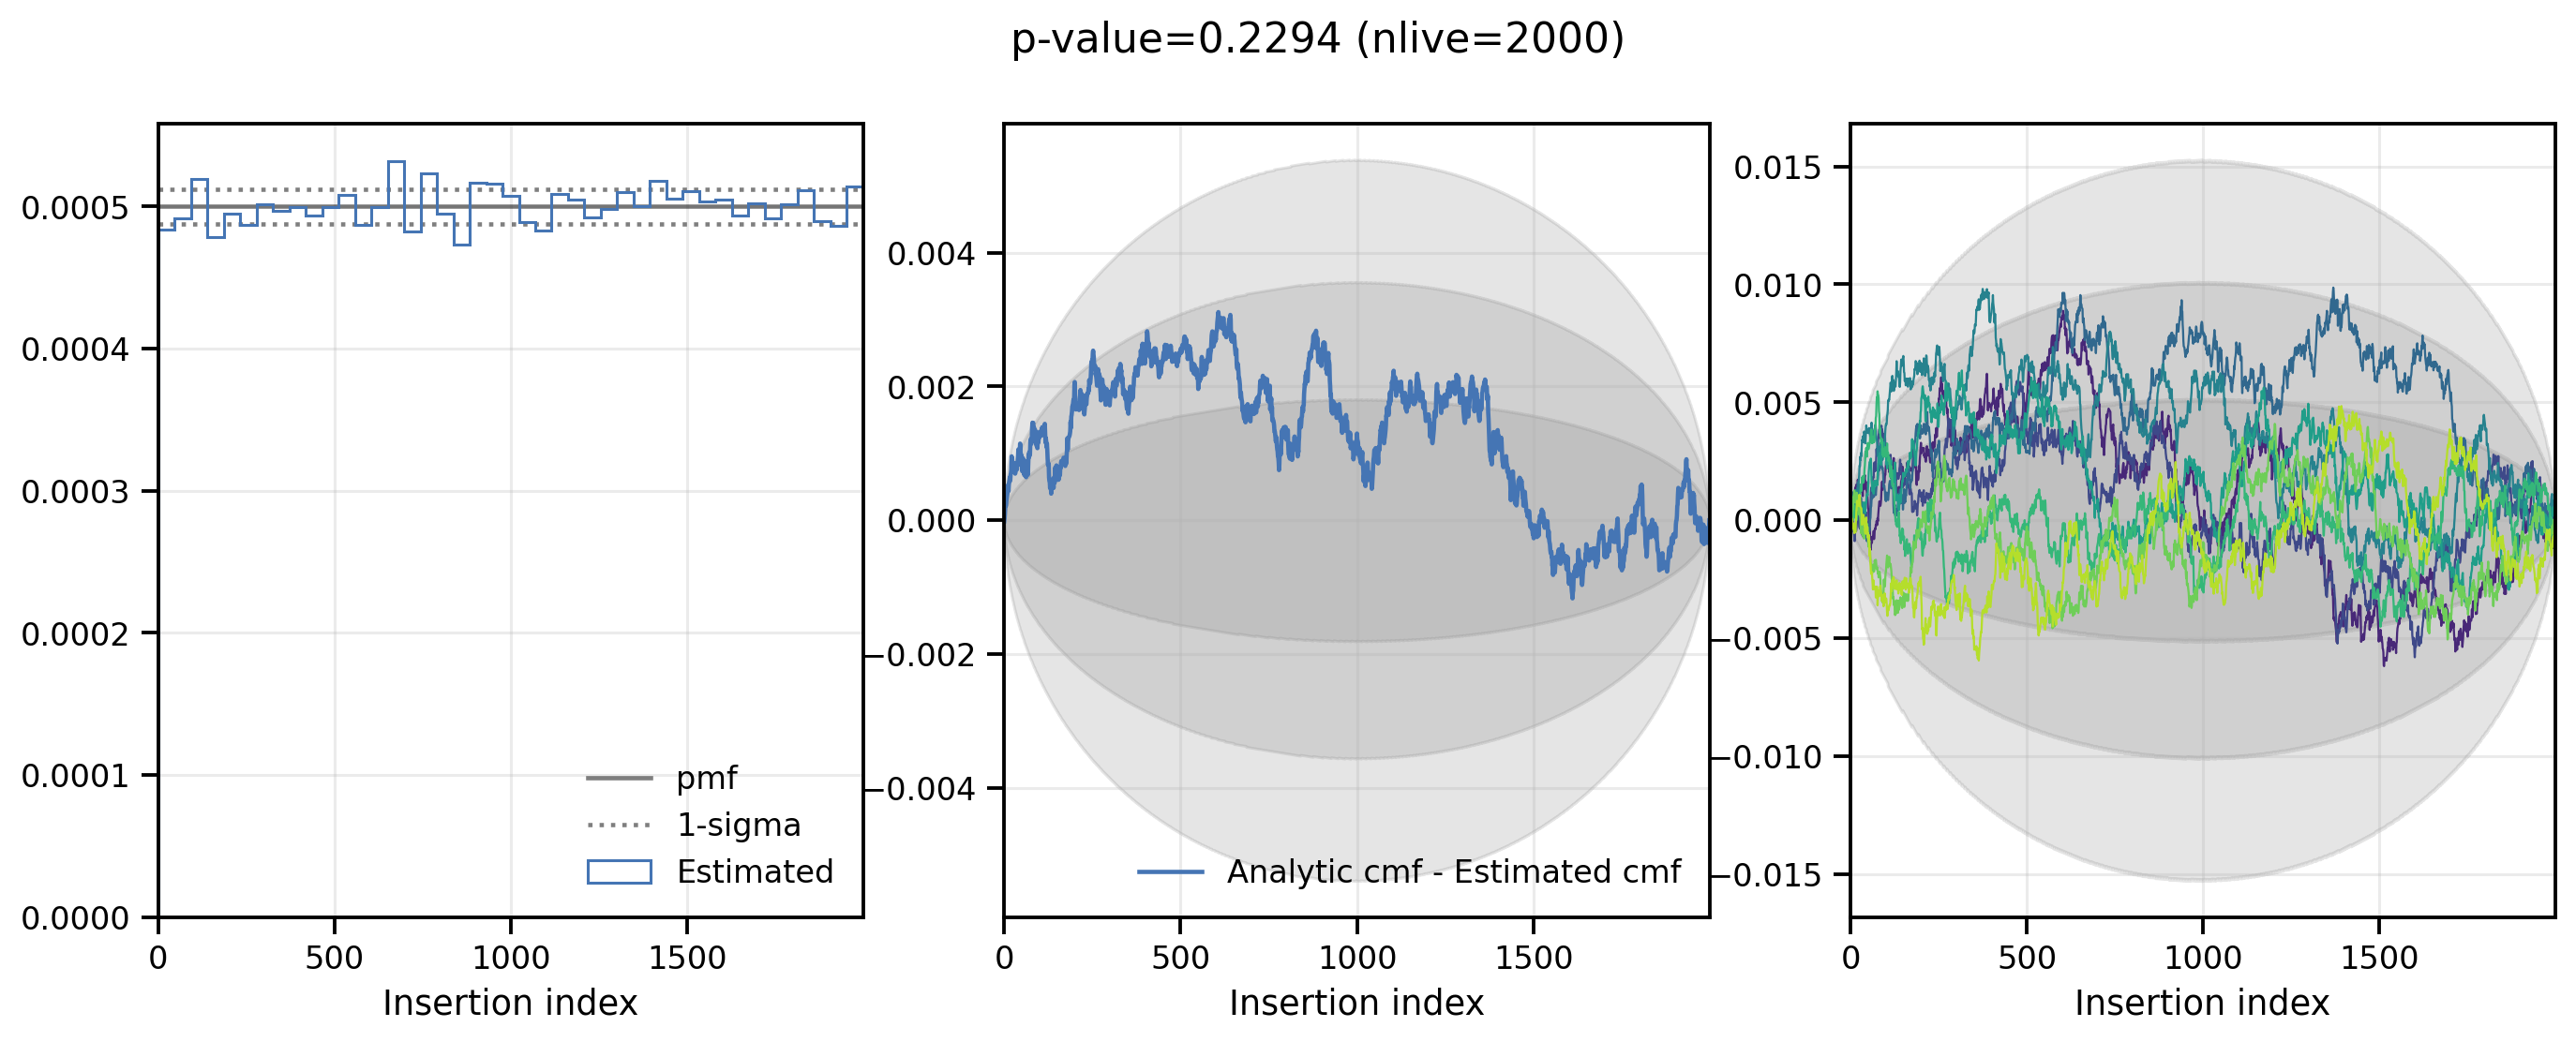
\includegraphics[width=\linewidth]{../figures/task5_subtask2/14_five_day_nessai_insertion_indices.png}
    \caption{5-day insertion-index}
  \end{subfigure}
  \caption{NESSAI insertion-index 诊断。两次运行的 KS \(p\) 值均未显示明显偏离。}
\end{figure}

\begin{figure}[H]
  \centering
  \begin{subfigure}{0.48\textwidth}
    \centering
    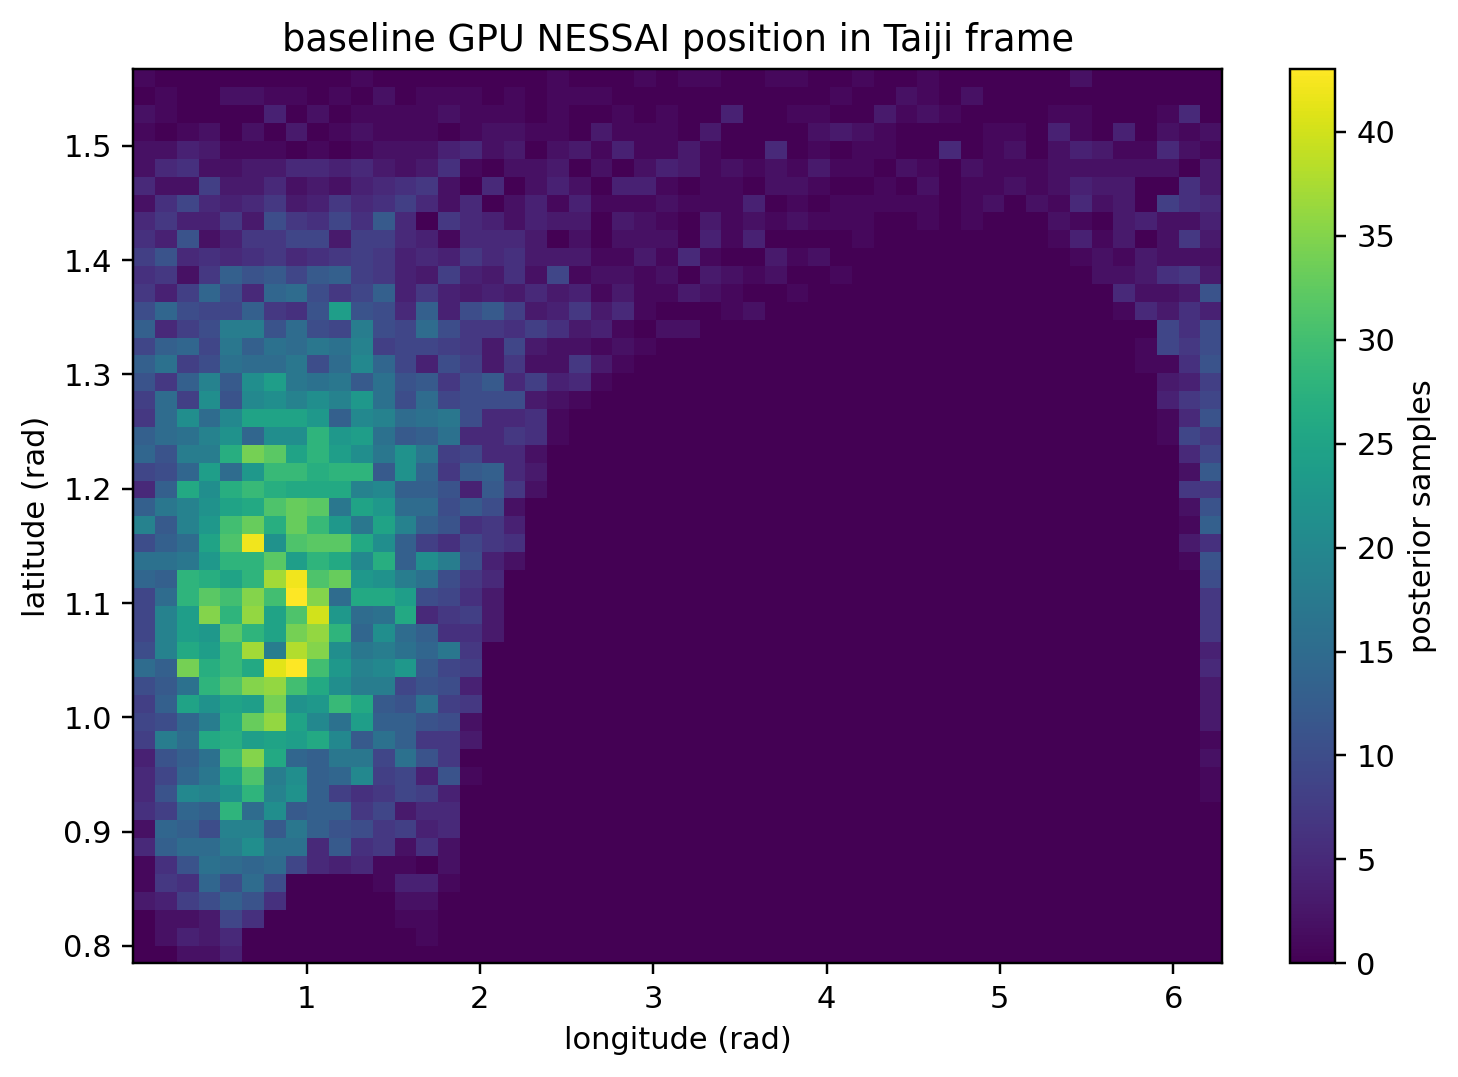
\includegraphics[width=\linewidth]{../figures/task5_subtask2/09_baseline_taiji_frame_sky.png}
    \caption{baseline Taiji frame}
  \end{subfigure}
  \hfill
  \begin{subfigure}{0.48\textwidth}
    \centering
    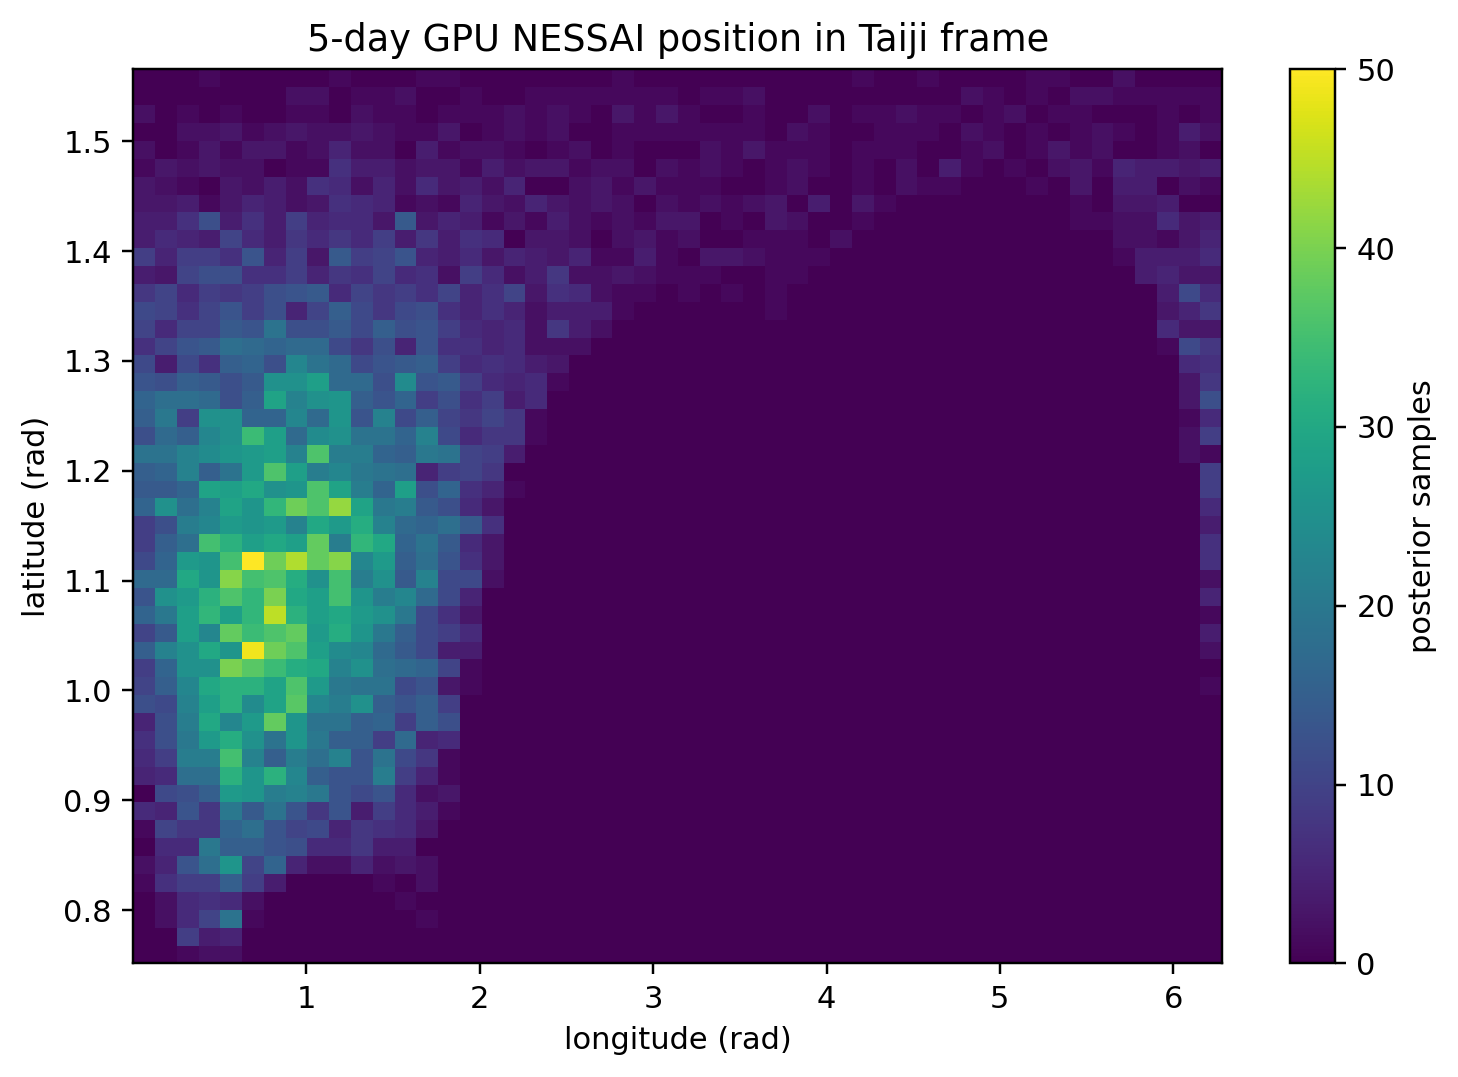
\includegraphics[width=\linewidth]{../figures/task5_subtask2/10_five_day_taiji_frame_sky.png}
    \caption{5-day Taiji frame}
  \end{subfigure}
  \caption{后验样本在 Taiji frame 中的天区分布。图中双峰结构反映天区反射简并。}
\end{figure}

\section{对关键知识点的理解}

\paragraph{为什么要做傅立叶变换？}
空间引力波信号是长时标 chirp 信号，噪声也强烈依赖频率。频域表达使得噪声加权
内积、PSD 校正和频带裁剪都变得直接。贝叶斯似然本质上就是“数据与模板之差”
在噪声加权频域中的二次型。

\paragraph{为什么 MBHB 参数相关性强？}
质量、合并时间和相位共同控制相位演化；距离、倾角和偏振共同控制振幅投影；
天区和探测器轨道调制共同决定 Doppler 相位。因此 corner 图中出现质量--自旋、
距离--倾角、天区--偏振等相关性是合理的，不应被误解为数值错误。

\paragraph{为什么 NESSAI 比单纯 MCMC 更适合本任务？}
子任务二不仅要给出后验，还要理解证据和采样诊断。NESSAI 作为嵌套采样器可以
同时提供 \(\log Z\)、后验样本和 insertion-index 诊断；normalising flow proposal
又能在高维复杂后验中提高提出新 live point 的效率。对本仓库而言，真正的加速来自
“杂频似然降低单次似然成本”和“GPU 向量化批量评估”，NESSAI 则保证统计推断形式
仍符合任务要求。

\paragraph{为什么 \(\Delta \log Z\) 不能跨窗口当作 Bayes factor？}
Bayes factor 只在同一数据、不同模型之间有直接意义。baseline 和 5-day 运行使用
的是不同时间段数据，因此 \(\log Z\) 的绝对值受数据长度、信号能量和噪声实现影响。
本报告只把各自的 \(\log Z\) 当作运行内部的证据和收敛摘要，不把二者差值解释为
“5-day 模型更受支持”。

\paragraph{为什么单次注入不能做 P--P 检验？}
P--P 检验需要一组独立注入，统计真实参数在后验分布中的累计概率是否服从均匀分布。
NESSAI 论文使用多注入集合验证无偏性；本任务只有一个 TDC 注入，因此只能报告
insertion-index、边界检查、trace/logX--logL 等单次运行诊断。

\section{与近两年开放获取文献的联系}

近两年 MBHB 推断研究呈现出两条趋势。第一条是继续强化 LISA/Taiji 网络对外禀参数
的约束能力。Gao 等人的 TianQin--LISA Bayesian parameter estimation 工作指出，
空间探测器网络可以显著改善外禀参数测量，但参数简并和信号覆盖阶段仍可能带来偏差。
这与本仓库中天区/距离/倾角的复杂后验形态一致。

第二条是快速推断方法成为核心问题。Vílchez 与 Sopuerta 使用 Sequential Neural
Likelihood 研究 MBHB 快速参数估计，Jan 等人将 RIFT 框架适配到 LISA MBHB 推断，
都说明长时标空间信号的传统逐点评估成本很高，需要似然加速、并行化或机器学习辅助。
本仓库采用的 GPU 杂频似然 + NESSAI 路线正处在这一技术脉络中：它没有用神经网络
替代后验，而是保留嵌套采样，同时降低每次似然评估成本。

\section{结论}

通过本仓库 notebook 2 的全量运行，可以形成如下理解：
\begin{itemize}
  \item 空间引力波数据分析的基础是 TDI 通道、FFT、PSD 和噪声加权频域似然。
  \item MBHB 信号的参数恢复不仅是数值拟合，更受探测器轨道调制和几何简并控制。
  \item NESSAI 提供了适合子任务二要求的贝叶斯后验、证据和诊断框架。
  \item GPU 杂频似然没有改变统计问题，而是把 Example 4 的全量 NESSAI 路线压缩到
  分钟级运行时间，使结果可复现、可诊断、可提交。
  \item 当前结果可信，但其科学边界需要明确：反射解是主要后验支；跨窗口
  \(\log Z\) 不作 Bayes factor；单注入不能替代 P--P 群体验证。
\end{itemize}

\begin{thebibliography}{9}

\bibitem{trianglebbh}
Triangle Data Center.
\newblock \emph{Triangle-BBH: \path{Examples/4_TDC_Verification_MBHB_Search_and_Estimation(CPU).ipynb}}.
\newblock GitHub repository, accessed 2026-06-12.
\newblock \url{https://github.com/TriangleDataCenter/Triangle-BBH}.

\bibitem{taiji-data-challenge}
Z. Ren, T. Zhao, Z. Cao, Z.-K. Guo, W.-B. Han, H.-B. Jin, and Y.-L. Wu.
\newblock Taiji Data Challenge for Exploring Gravitational Wave Universe.
\newblock \emph{Frontiers of Physics} 18, 64302 (2023).
\newblock arXiv:2301.02967, \url{https://arxiv.org/abs/2301.02967}.

\bibitem{nessai}
M. J. Williams, J. Veitch, and C. Messenger.
\newblock Nested Sampling with Normalising Flows for Gravitational-Wave Inference.
\newblock \emph{Physical Review D} 103, 103006 (2021).
\newblock arXiv:2102.11056, \url{https://arxiv.org/abs/2102.11056}.

\bibitem{tianqin-lisa-mbhb}
J. Gao, Y.-M. Hu, E.-K. Li, J.-D. Zhang, and J. Mei.
\newblock Bayesian parameter estimation of massive black hole binaries with TianQin-LISA.
\newblock Open-access preprint, arXiv:2401.12813 (2024).
\newblock \url{https://arxiv.org/abs/2401.12813}.

\bibitem{sbi-mbhb}
I. M. Vílchez and C. F. Sopuerta.
\newblock Efficient Massive Black Hole Binary parameter estimation for LISA using Sequential Neural Likelihood.
\newblock Open-access preprint, arXiv:2406.00565 (2024).
\newblock \url{https://arxiv.org/abs/2406.00565}.

\bibitem{rift-lisa}
A. Jan, R. O'Shaughnessy, D. Shoemaker, and J. Lange.
\newblock Adapting a novel framework for rapid inference of massive black hole binaries for LISA.
\newblock Open-access preprint, arXiv:2410.15542 (2024).
\newblock \url{https://arxiv.org/abs/2410.15542}.

\end{thebibliography}

\end{document}
